\documentclass[11pt,a4paper]{article}

\usepackage[margin=2.2cm]{geometry}
\usepackage[utf8]{inputenc}
\usepackage[T1]{fontenc}
\usepackage{graphicx}
\usepackage{booktabs}
\usepackage{array}
\usepackage{amsmath}
\usepackage{hyperref}
\usepackage{enumitem}
\usepackage{titlesec}

\titlespacing*{\section}{0pt}{1.4em}{0.6em}
\titlespacing*{\subsection}{0pt}{1.1em}{0.5em}

\title{\large Optimal Bayes Classification -- Card Suit Recognition\\[4pt]
\normalsize EPART Laboratory \#2 \\ \textit{(MATLAB)}}
\author{Alicja Misterka \\
325045, lab group 102}
\date{12.11.2026}

\begin{document}
\maketitle
\vspace{-2.2em}

\section{Method summary}

Three probability-density estimators were implemented and plugged into the
generic Bayes classifier (\texttt{bayescls.m}):
\begin{itemize}
  \item \texttt{pdf\_indep.m}: Gaussian model with independent features (the
    class density is a product of one-dimensional normal densities),
  \item \texttt{pdf\_multi.m}: multivariate Gaussian model,
  \item \texttt{pdf\_parzen.m}: non-parametric Parzen-window estimator with a
    Gaussian kernel (a product of one-dimensional kernels); following the
    assignment, the kernel width for a class with $n$ training samples is
    $h_n = h_1/\sqrt{n}$.
\end{itemize}
All three functions were verified on the supplied \texttt{pdf\_test.txt} set
(2 classes, 2 features, 20 samples) and reproduced the reference density values
exactly.

The card-suit data use the 7 Hu moment invariants as features. The original
4 class labels (clubs, diamonds, hearts, spades) were expanded to 8 classes to
account for the two print methods (with / without printing raster): the four
suits printed with one method form classes 1--4 and the same suits printed
with the other method form classes 5--8.

\section{Data cleaning (Q1)}

The mean and the median of every feature were compared on the raw training set
(1824 samples). Several features showed mean--median differences of 2--4
orders of magnitude (e.g.\ Hu-5: mean $\approx 79.7$, median $\approx 0.0000$,
std $\approx 3400$) --- a clear sign of outliers rather than natural skew.
Sorting each feature column and inspecting its extreme values showed that two
samples were contaminated:

\begin{itemize}[leftmargin=1.4em]

\item \textbf{Row 186} --- its features are far larger than in any other
sample (e.g.\ Hu-1 $= 5.12$ vs.\ the next-highest $0.21$; Hu-5 $= 1.45\cdot10^{5}$
vs.\ $\approx 0$), whereas the neighbouring rows 185 and 187 are completely
ordinary. It is an isolated corrupted sample, not a genuine one.

\item \textbf{Row 642} --- all 7 feature values are exactly \texttt{0} (a
degenerate sample, probably derived from a blank/empty image region), again
inconsistent with its neighbours.

\end{itemize}

Both rows were dropped from the training set (1824 $\to$ 1822 samples).
Re-running the identical extreme-value scan afterwards showed no isolated
jumps, and the mean and median of each feature came much closer together, so
the procedure was stopped after a single pass. The test set was scanned in the
same way and no analogous outliers were found; thus, as instructed in the
assignment, it was left unchanged --- only the training set was cleaned.

\section{Feature selection (Q2)}

Rather than picking a pair of the 7 Hu moments by eye, every one of the
$\binom{7}{2} = 21$ possible feature pairs was scored by the average test
error of the \texttt{indep} and \texttt{multi} classifiers (equal priors).
Hu moments \textbf{1 and 3} were the clear winner:

\begin{table}[h!]
\centering
\begin{tabular}{@{}cll@{}}
\toprule
Rank & Hu moments & Avg.\ error \\
\midrule
1 & 1 \& 3 & 1.56\% \\
2 & 2 \& 3 & 2.11\% \\
3 & 1 \& 4 & 6.77\% \\
\bottomrule
\end{tabular}
\end{table}

\begin{figure}[h!]
\centering
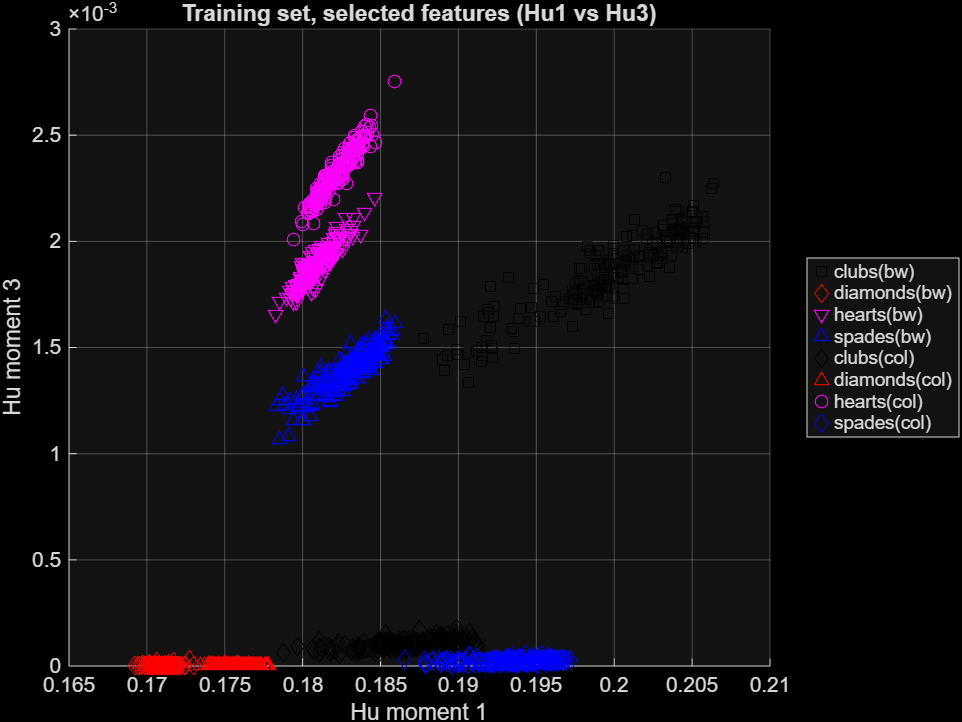
\includegraphics[width=0.62\linewidth]{fig_features.png}
\caption{Training set on the selected features (Hu-1, Hu-3); colour = suit,
shape = print method.}
\end{figure}

All further experiments use this feature pair, with equal a priori
probabilities of 0.125 for every class (note: since all 8 priors are equal,
multiplying every class's density by the same constant has no effect on the
arg-max decision --- the a priori term was still passed to
\texttt{bayescls} to match the assignment statement, but Q2--Q4's numbers
would be identical without it).

\textbf{Baseline error rates} (full cleaned training set, Parzen width
$h_1 = 0.001$):

\begin{table}[h!]
\centering
\begin{tabular}{@{}lccc@{}}
\toprule
Classifier & indep & multi & parzen \\
\midrule
Test error & 2.63\% & 0.49\% & 2.41\% \\
\bottomrule
\end{tabular}
\end{table}

The multivariate classifier wins clearly --- Fig.~1 shows the classes form
elongated, correlated clusters (diagonal bands), which \texttt{pdf\_multi}
can model via the feature covariance but \texttt{pdf\_indep} cannot (it
assumes axis-aligned Gaussians). The confusion matrix for \texttt{multi}
shows the (small) residual errors spread thinly over several classes rather
than concentrated in one confusable pair --- consistent with Fig.~1, where
all 8 clusters are mostly well separated with only minor overlap at cluster
edges.

\section{Effect of training-set size (Q3)}

Using \texttt{reduce.m}, every class was reduced to the same fraction of its
training samples (10\% / 25\% / 50\%; the samples are drawn independently within
each class, and only the training set is reduced). The draw was repeated 10
times per fraction to average out sampling noise.

\begin{table}[h!]
\centering
\begin{tabular}{@{}lccc@{}}
\toprule
Train fraction & indep (mean $\pm$ std) & multi (mean $\pm$ std) & parzen (mean $\pm$ std) \\
\midrule
10\%  & 2.79\% $\pm$ 0.42\% & 0.95\% $\pm$ 0.30\% & 9.28\% $\pm$ 1.54\% \\
25\%  & 2.86\% $\pm$ 0.17\% & 0.75\% $\pm$ 0.19\% & 5.53\% $\pm$ 0.46\% \\
50\%  & 2.64\% $\pm$ 0.21\% & 0.61\% $\pm$ 0.11\% & 4.09\% $\pm$ 0.42\% \\
100\% (ref.) & 2.63\% & 0.49\% & 2.41\% \\
\bottomrule
\end{tabular}
\end{table}

\begin{figure}[h!]
\centering
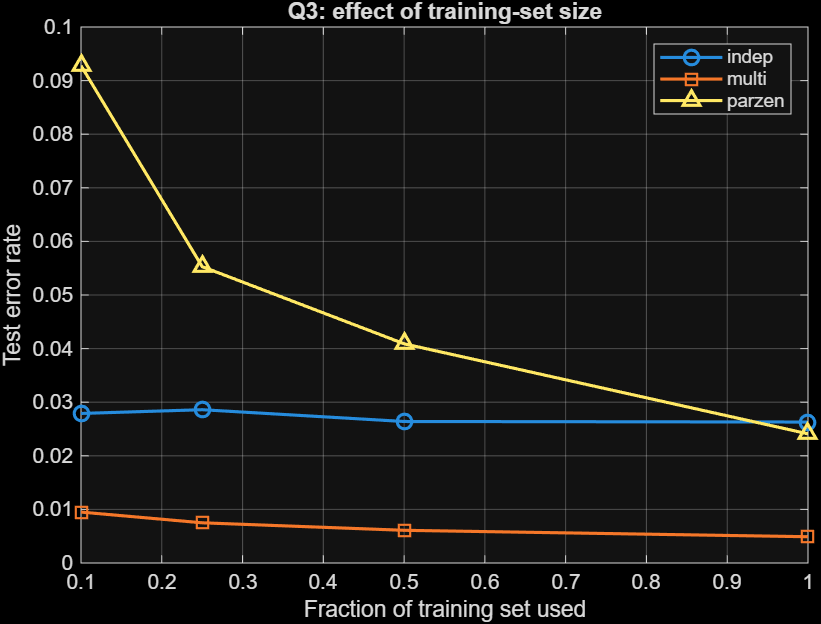
\includegraphics[width=0.58\linewidth]{fig_trainsize.png}
\caption{Test error vs.\ fraction of training data used, per classifier.}
\end{figure}

This matches expectations: the two \emph{parametric} classifiers only need
to estimate a mean (and, for \texttt{multi}, a $2\times2$ covariance) per
class, which stabilises quickly --- even 10\% of the data ($\approx$23
samples/class) is almost enough. The \emph{non-parametric} Parzen estimator
has no such shortcut: its density estimate is literally built from the
training samples themselves, so cutting the sample count directly thins out
the density estimate and error roughly doubles going from 50\% $\to$ 10\% of
the data.

\section{Effect of Parzen window width (Q4)}

The window width $h_1$ was varied over the whole required interval
$\langle 0.0001, 0.01\rangle$ (full cleaned training set, \texttt{parzen} only):

\begin{table}[h!]
\centering
\begin{tabular}{@{}lccccc@{}}
\toprule
$h_1$ & 0.0001 & 0.0005 & 0.001 & 0.005 & 0.01 \\
\midrule
Error & 2.85\% & \textbf{1.70\%} & 2.41\% & 7.95\% & 13.93\% \\
\bottomrule
\end{tabular}
\end{table}

\begin{figure}[h!]
\centering
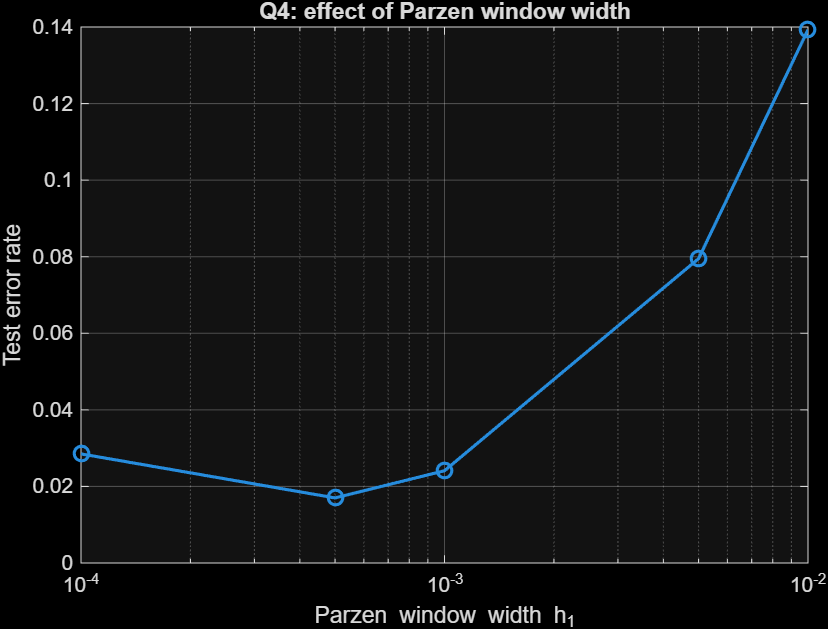
\includegraphics[width=0.55\linewidth]{fig_parzen_width.png}
\caption{Test error vs.\ Parzen window width $h_1$ (log scale).}
\end{figure}

There is a clear sweet spot around $h_1 \approx 0.0005$: too narrow a window
(0.0001) makes the density estimate noisy and overly peaked on individual
training samples; too wide a window (0.005--0.01) oversmooths the estimate
until it blurs together density from neighbouring, different classes, which
collapses classification quality (13.9\% error at $h_1 = 0.01$). This is the
classic bias/variance trade-off of kernel density estimation.

\section{Asymmetric a priori probabilities (Q5)}

As instructed, only the \textbf{test set} was reduced --- red suits
(diamonds, hearts, and their two print-method variants) were cut to 50\%,
simulating an operating scenario where red cards are rarer. This was
repeated 10 times; classifiers were trained once on the full (cleaned)
training set. The black-favouring priors were
$(0.165, 0.085, 0.085, 0.165, 0.165, 0.085, 0.085, 0.165)$ for classes 1--8,
i.e.\ twice as high for the black suits (classes 1, 4, 5, 8).

\begin{table}[h!]
\centering
\begin{tabular}{@{}lccc@{}}
\toprule
A priori & indep & multi & parzen \\
\midrule
Equal (0.125 each) & 2.09\% $\pm$ 0.15\% & 0.38\% $\pm$ 0.06\% & 2.82\% $\pm$ 0.09\% \\
Black-favouring (0.165 / 0.085) & 2.12\% $\pm$ 0.16\% & 0.38\% $\pm$ 0.06\% & 2.82\% $\pm$ 0.09\% \\
\bottomrule
\end{tabular}
\end{table}

Changing the priors to match the (now imbalanced) class ratios in the test
set made essentially \textbf{no difference} (well within one standard
deviation for all three classifiers). This makes sense given how separable
the classes already are on this feature pair (sub-1\% error for
\texttt{multi}): the likelihood ratio between the true class and any
competitor is overwhelmingly large almost everywhere, so multiplying by a
factor of $\sim$2 prior shift is not enough to flip any decisions. Priors
only start to matter when the likelihoods of two classes are close ---
which practically never happens here.

The absolute errors in the ``equal priors'' row differ from the baseline in
Section~3 simply because the test set is different: halving the red suits shifts
the weight towards the black classes. Interestingly, the error of \texttt{parzen}
went \emph{up} (2.41\% $\to$ 2.82\%) while those of \texttt{indep} and
\texttt{multi} went down. This implies that \texttt{parzen} makes relatively
more mistakes on black suits than on red ones, and \texttt{indep} the opposite.

\section{1-NN classifier and normalization (Q6)}

\texttt{std(train)} on the two selected features gives 0.0088 for Hu-1 and
0.0010 for Hu-3 --- roughly a $9\times$ difference in scale. Since 1-NN
decides purely by Euclidean distance, the larger-scale feature (Hu-1) would
dominate the distance calculation and effectively drown out Hu-3's
contribution. Both train and test sets were therefore z-score normalized
using statistics computed on the training set only. The classifier
(\texttt{cls1nn.m}) was evaluated directly on the test set, without
leave-one-out, as the test set is large enough.

\begin{table}[h!]
\centering
\begin{tabular}{@{}lcc@{}}
\toprule
 & Raw features & Normalized features \\
\midrule
1-NN test error & 1.75\% & \textbf{0.49\%} \\
\bottomrule
\end{tabular}
\end{table}

Normalizing more than triples the accuracy (1.75\% $\to$ 0.49\% error),
confirming the scale mismatch was indeed hurting the distance-based
classifier --- exactly as the std comparison predicted. With
normalization, 1-NN reaches the same error rate as the best Bayes
classifier (\texttt{multi}, also 0.49\%), which is a sensible outcome: with
only two well-separated, now-comparable-scale features, the nearest
neighbour is almost always the sample's own, correct class.

\section{Conclusions}

\begin{itemize}[leftmargin=1.4em]
  \item Two corrupted training samples were found and removed; without this
    cleaning step the estimated class means/covariances --- and hence every
    classifier built on them --- would have been distorted.
  \item Hu moments 1 and 3 separate the 8 classes far better than other
    pairs, reducing baseline error from $\sim$26\% (an arbitrary placeholder
    pair) to under 3\% for every classifier.
  \item \texttt{pdf\_multi} consistently outperforms \texttt{pdf\_indep}
    because the classes' feature covariance is informative (correlated,
    elongated clusters) --- the independence assumption throws that away.
  \item Parametric classifiers are far more data-efficient than the
    non-parametric Parzen estimator, which needs the full training set to
    match the independent-Gaussian model and stays well behind
    \texttt{multi} even at its best width (1.70\% vs.\ 0.49\%). The fact that
    the Gaussian model \texttt{multi} beats the more flexible Parzen
    estimator indicates that the classes are very close to Gaussian on this
    feature pair.
  \item The Parzen width is a genuine bias/variance knob with a clear
    optimum; neither extreme of the required $\langle 0.0001, 0.01\rangle$
    range is a good choice here.
  \item A priori probabilities only matter when classes are hard to tell
    apart from the data alone --- with features this separable, they had
    virtually no effect.
  \item Feature scale matters a great deal for distance-based classifiers;
    z-score normalization fixed a real, predictable weakness of 1-NN on
    this data.
  \item \textbf{Expected vs.\ unexpected.} Most results agreed with
    expectations (more data helps the non-parametric classifier most,
    wide Parzen windows oversmooth, normalization helps 1-NN). The
    less obvious findings were that the priors made no measurable
    difference, that plain 1-NN on normalized features matched the best
    Bayes classifier, and that halving the red test samples moved the
    error of \texttt{parzen} in the opposite direction to the parametric
    classifiers (Section~6).
\end{itemize}

\end{document}